\documentclass{article}
\usepackage{graphicx}
\usepackage[a4paper, total={7in, 12in}]{geometry}
\bibliographystyle{plain}

\title{Is Florida Warming?} % Sets article title
\author{Jooyoung Ser} % Sets authors name
\date{\today} % Sets date for publication as date compiled

% The preamble ends with the command \begin{document}
\begin{document} % All begin commands must be paired with an end command somewhere

\maketitle % creates title using information in preamble (title, author, date)
    
	%New section is created
\section{Introduction}
	%Plain text is just written directly in this document like this:
	Florida Keys, a coral cay archipelago, located off the southern coast of Florida houses many coral reefs. Global warming has been known to cause coral bleaching so it is important to monitor climatic changes in Florida \cite{kuffner2015century}. This document shows the results of a practical that attempts to answer the question: "Is Florida getting warmer?". The analysis was done on 20th Century temperature data from Key West, Florida. A permutation analysis was conducted as the measurements were in successive time-points in a time series which make them not independent. The permutation analysis was run using R code and was simulated 1000 times. The results of these simulations were then compared with the observed correlation coefficient of the Florida temperature data.
	
\section{Results}
	Correlation coefficients were calculated in R using Pearson's formula:
		\begin{center}
			\begin{equation} 
				r = \frac{ \sum_{i=1}^{n}(x_i-\bar{x})(y_i-\bar{y}) }{%
				\sqrt{\sum_{i=1}^{n}(x_i-\bar{x})^2}\sqrt{\sum_{i=1}^{n}(y_i-\bar{y})^2}}
			\end{equation}
		\end{center}
	\begin{figure}[h!]
		\begin{center}
			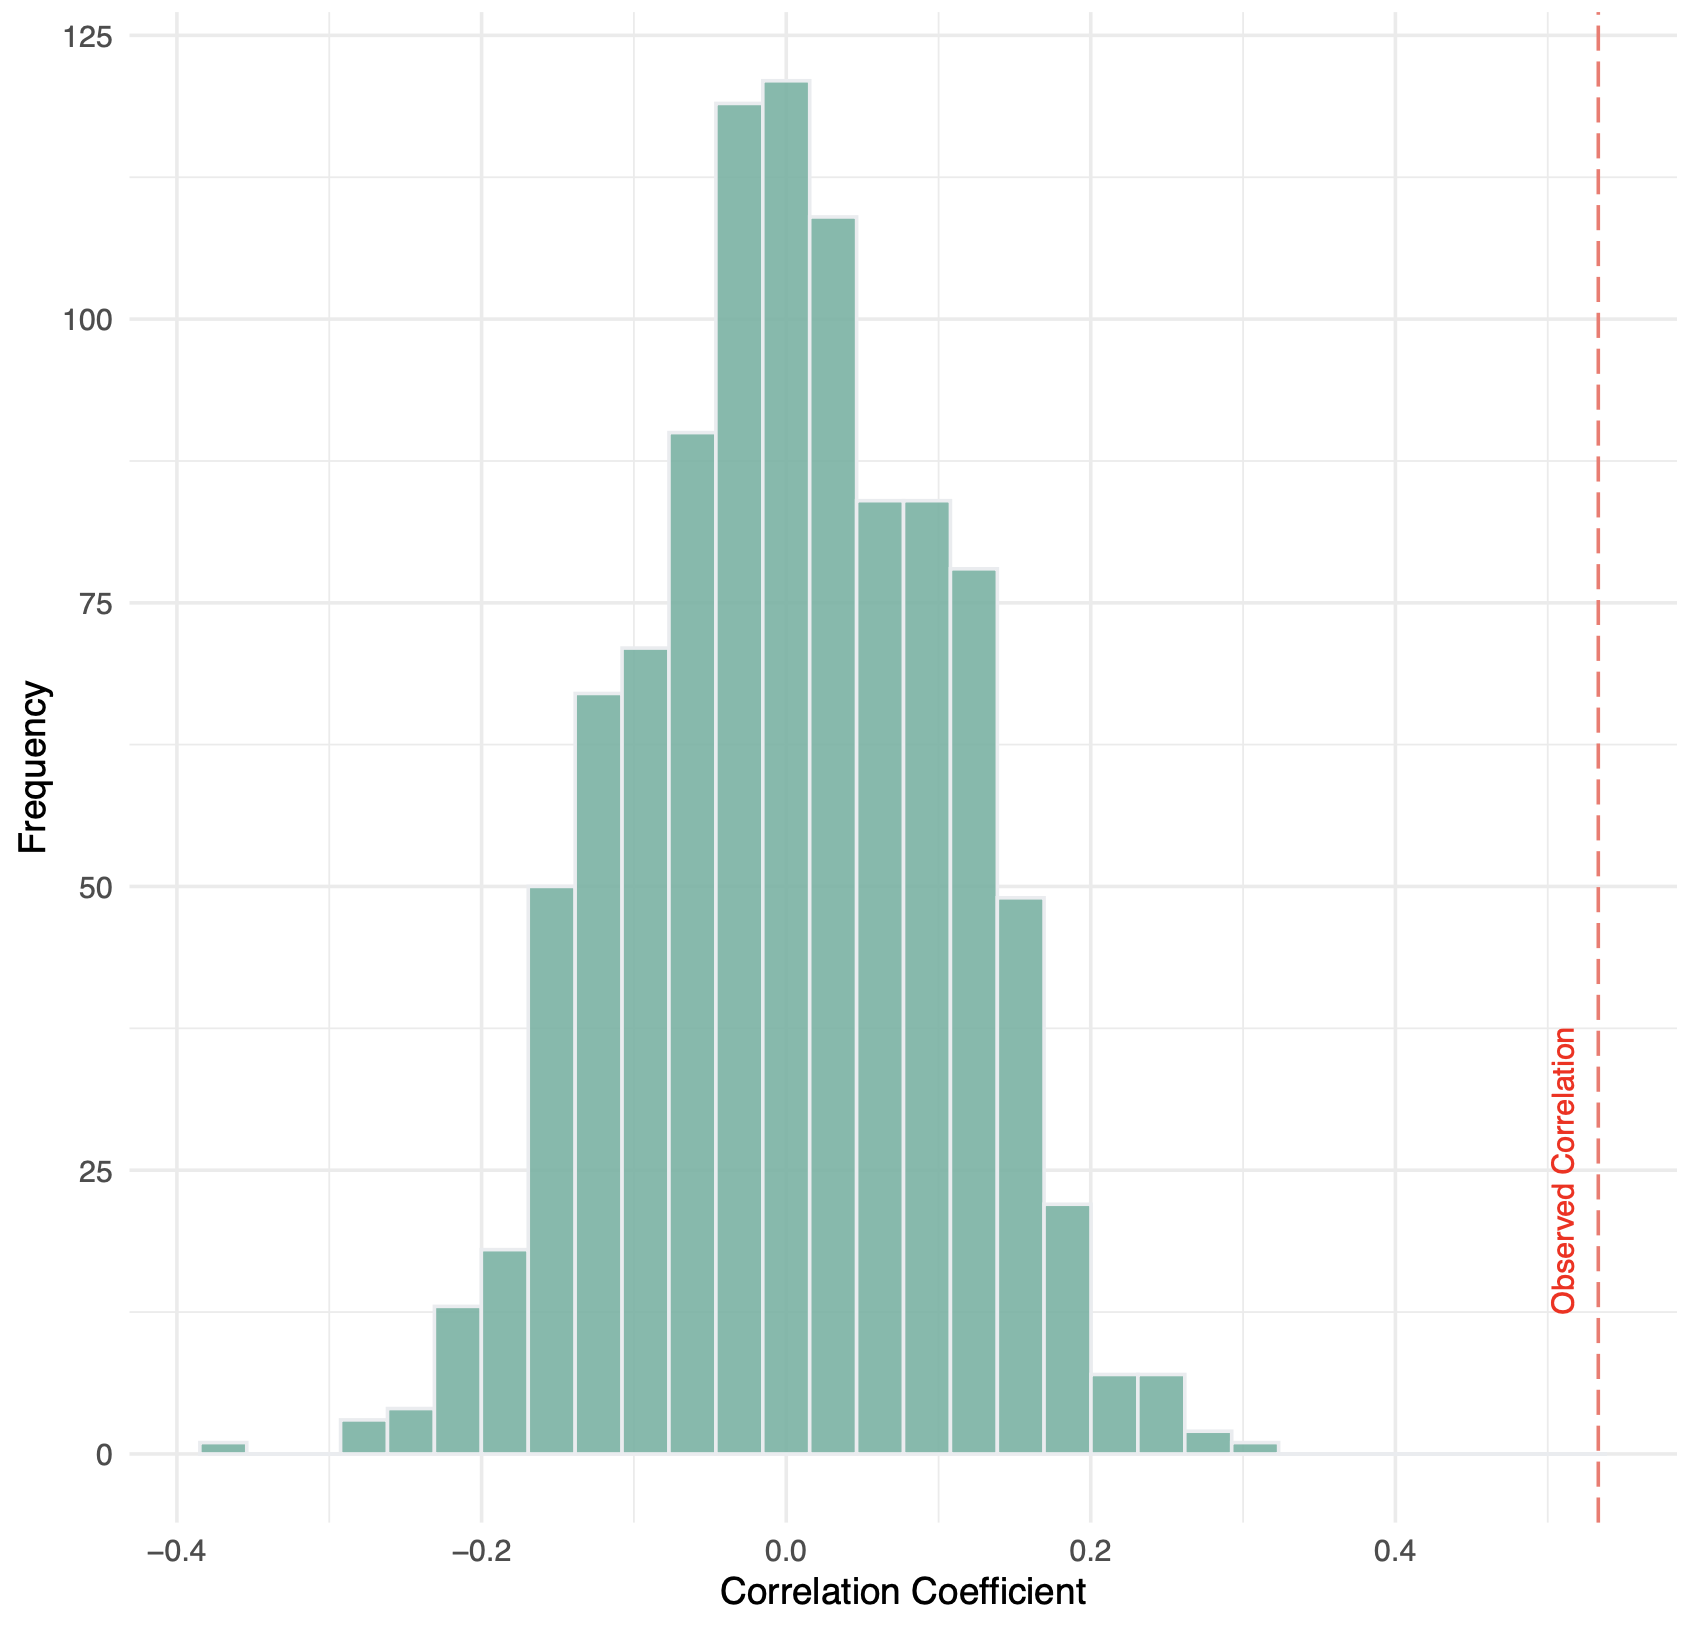
\includegraphics[width=90mm]{../results/florida_histogram.png}
		\end{center}
		\caption{Observed Correlation Compared With Random Permutations.}
		\label{fig1}
	\end{figure}

	Temperature increased statisitcally significantly in the 20th Century in Florida Keys which is shown in Figure 1. The histogram shows the correlation coefficients of all 1000 analyses of the randomly shuffled data. None of these correlation coefficients exceed the observed correlation coefficient of 0.533 (3 s.f.), shown on the figure as a red vertical line. This suggests that Florida is in fact getting warmer. 

	%Add bibliography at the end of document	
	\bibliography{floridabib}
\end{document} % This is the end of the document